\documentclass{ximera}

\newcommand{\RR}{\mathbb R}
\renewcommand{\d}{\,d}
\newcommand{\dd}[2][]{\frac{d #1}{d #2}}
\renewcommand{\l}{\ell}
\newcommand{\ddx}{\frac{d}{dx}}
\newcommand{\dfn}{\textbf}
\newcommand{\eval}[1]{\bigg[ #1 \bigg]}


\author{Jim Talamo}
\license{Creative Commons 3.0 By-NC}


\outcome{Set up an integral to compute a volume of a solid with known cross-sections}

\begin{document}

\begin{exercise}

Suppose that $\sum_{k=1}^{\infty} a_k =4$ and it is known that $\sum_{k=1}^{15} a_k =1$.  

Is it possible to define a sequence of remainders?
\begin{multipleChoice}
\choice[correct]{Yes, because $\sum_{k=1}^{\infty} a_k$ converges.}
\choice{No, because we do not have a formula for $s_n$ in general.}
\end{multipleChoice}

Which term in the sequence of remainders $\{r_n\}_{n=1}$ can we find?

\begin{multipleChoice}
\choice{$r_{14}$}
\choice[correct]{$r_{15}$}
\choice{$r_{14}$}
\end{multipleChoice}

\begin{exercise}

Which of the following expressions gives $r_{15}$?
\begin{multipleChoice}
\choice{$\sum_{k=1}^{\infty} a_k$}
\choice{$\sum_{k=1}^{14} a_k$}
\choice{$\sum_{k=1}^{15} a_k$}
\choice[correct]{$\sum_{k=1}^{16} a_k$}
\end{multipleChoice}

From the given information, we find that $r_{15} = \answer{3}$.

\begin{hint}
Note $\sum_{k=1}^{\infty} a_k = r_n+s_n$ for every $n\geq 1$. We know $\sum_{k=1}^{\infty} a_k= 4$ and $s_{15} = \sum_{k=1}^{15} a_k =1$, so this allows us to solve for $r_{15}$.

\end{hint}
\begin{feedback}
Recall that we can always define a sequence of remainders if we have a \emph{convergent} series, and we can split such a series up in the following way.

\begin{image}
  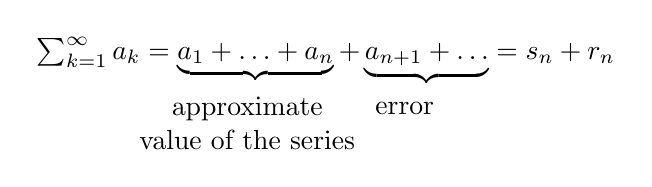
\begin{tikzpicture}
        \node at (0,0) {
          $ \sum_{k=1}^{\infty} a_k=\underbrace{a_1+\ldots +a_n}+ \underbrace{a_{n+1}+ \ldots} = s_n+r_n$};
        \node at (1,-.6) { error};
       
        \node at (-1,-.6) {approximate };
        \node at (-1,-1) {value of the series };
                
      \end{tikzpicture}
  \end{image}
  
  The lower index in the sum for $r_n$ always starts at $n+1$ so we can write the series $ \sum_{k=1}^{\infty} a_k$ as $s_n +r_n$.
  
  We do this because we want to approximate the \emph{infinite} series $\sum_{k=1}^{\infty} a_k$ by the \emph{finite} one $ \sum_{k=1}^{n} a_k$.  The remainder term $r_n$ will tell us the error made using this approximation.
\end{feedback}


\end{exercise}

\end{exercise}
\end{document}